When finishing with a training session for a machine learning model, we need to use different metrics to be able to tell how the model performed based on some testing data. For prediction models, we only consider the value returned by the \textit{loss function}, but evaluation of classification models can be presented with several metrics. In this section we present loss functions and optimizers, and how we evaluate the performance of our models using classification metrics and different ways of splitting up into training and testing data.

\subsection{Loss functions and Optimizers}

After defining a machine learning model, we \textit{compile} it so that it was ready to be \textit{fit} to the dataset. Compiling a model requires a \textit{loss function} and an \textit{optimizer}. The loss function is the function that evaluates how well the model \textit{models} the given data \cite{loss_functions}, and the optimizer is the function that attempts to lower the output of the loss function. 

For the first two objectives in this thesis, we use the loss function \textit{categorical crossentropy}, which calculates a probability over the number of classes supplied (number of classes equals the number of neurons in the output layer) \cite{cross_entropy}. In the third objective, we use a loss function called \textit{Mean Squared Error (MSE)}, which is measured as the average (mean) of squared difference between predictions and actual observations \cite{loss_functions}. The formula below is used to calculate the MSE, where $n$ is number of training samples, $i$ describes the current element in the samples, $y_i$ is true label for the current sample and $\hat{y}_i$ is the predicted label for the current sample.

\[ MSE = \frac{\sum_{i=1}^{n}(y_i-\hat{y}_i)^2}{n} \]

When choosing an optimizer, there are many different options available, but we chose an optimizer called \textit{Adam} for training all of our models. Adam is an algorithm for efficient stochastic gradient-based optimization \cite{adam}, and it is available as an optimizer function within the Keras framework \cite{keras_docs}. The reason for choosing Adam is, as described by Kingma, D. P. et al. \cite{adam}, efficient both considering memory usage and computationally. The hyper-parameters also require minimal tuning. Using a different optimizer can make the model fit the dataset at a different pace, which is something we experiment with in chapter \ref{chapter:training} (for the third objective). 

\subsection{Classification metrics}
In classification, accuracy is a metric that is commonly used. It makes sense to the human brain; telling a friend that has no experience in machine learning or data science that we have made our computer able to classify something with 98\% accuracy is something that they would understand. Other metrics include \textit{precision}, \textit{recall}, \textit{specificity} and \textit{F1 score} \cite{GarciaCeja2018_classification_bipolar}, which will be described below.

\subsubsection{Confusion matrix}

\begin{figure}[h]
  \begin{center}
    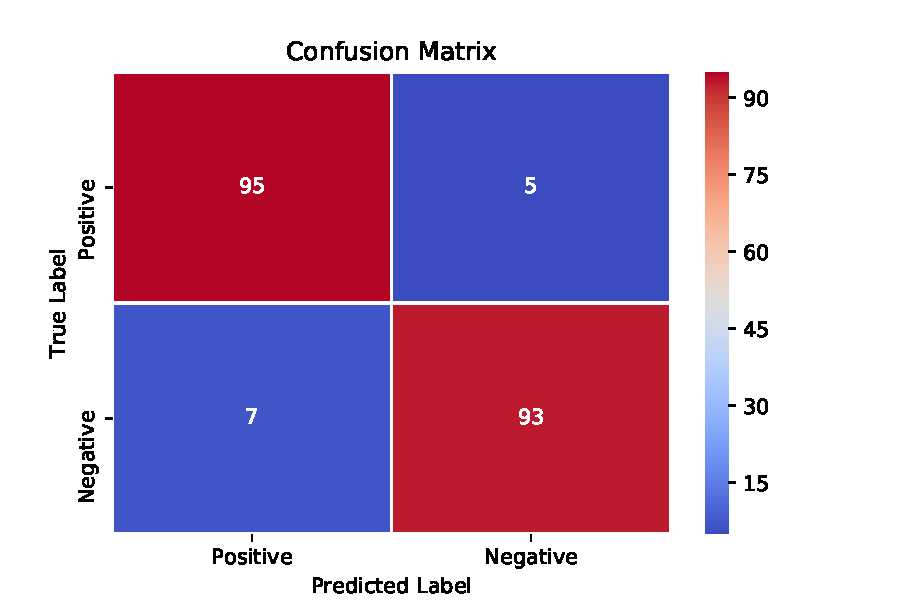
\includegraphics[height=8cm]{img/conf_matrix.pdf}
    \caption{Confusion Matrix Example: 95 True Positives, 93 True Negatives, 7 False Positives and 5 False Negatives}
    \label{figure:confusion_matrix_bipolar}
  \end{center}
\end{figure}

Figure \ref{figure:confusion_matrix_bipolar} shows a \textit{confusion matrix}. It is a visual metric for classification models in machine learning and is the basis for the other performance metrics. It can tell how well our model is performing by having correlation values for the different classes. Let us say we have 200 samples in our test data to use on our model that classifies control vs. condition group. 

A \textit{confusion matrix} for a good model would look like figure \ref{figure:confusion_matrix_bipolar}, with high numbers in \textbf{True Positive (TP)} and \textbf{True Negative (TN)} and as low numbers as possible in \textbf{False Positive (FP)} and \textbf{False Negative (FN)}. Having a high number in \textbf{True Positive} means that the model can classify that a participant is in the condition group if he or she is, and having a high number in \textbf{True Negative} means that the model can classify that a participant is in the control group if this is the case. The other cases, \textbf{False Positive} and \textbf{False Negative}, are where the model made a wrong classification, and therefore as close these numbers are to zero the better our model is.

\subsubsection{Accuracy}

\blockquote[\cite{ml_metrics}]{Accuracy is a good measure when the target variable classes in the data are nearly balanced.}

\[ \frac{TP + TN}{TP + TN + FN + FP} \]

When calculating the \textit{accuracy}, we sum up the correct predictions and divide that with the total number of predictions. For our example (\ref{figure:confusion_matrix_bipolar}), the \textit{accuracy} would be $ \frac{93 + 95}{93 + 95 + 5 + 7} = 0.94 $. It is a good metric to use for our example because the number of samples for each variable class is well balanced ($ 93+5=98 $ samples where \textbf{condition group} was the correct option, and $ 7+95=102 $ samples where \textbf{control group} was correct).

Terrible use of the \textit{accuracy} metric would be when one of the classes strongly dominates the samples. For example, if a model predicts \textbf{cancer} vs. \textbf{no cancer}, and the samples contain five people with cancer, and the 95 remaining people do not. The model would be terrible at predicting cancer and still have an accuracy score of $ 0.95 $ \cite{ml_metrics}.

\subsubsection{Precision} 

\[ \frac{TP}{TP + FP} \]

Precision operates entirely on the predicted positives, and it tells us how many \textbf{true positives} there is among \textbf{predicted positives} \cite{ml_metrics}. 

This performance metric is better to use on \textit{unbalanced} classes than accuracy. The \textit{cancer vs no cancer} example, assuming it predicts no-one to have \textbf{cancer}, would yield a precision score of $ \frac{5}{5+95} = 0.05 $. And our \textit{control vs condition} example would result in a precision score of $ \frac{93}{93+7} = 0.93 $.

\subsubsection{Recall}

\[ \frac{TP}{TP+FN} \]

\textit{Recall} is another useful performance metric. It tells us the relationship between \textbf{true positives} and \textbf{actual positives}, for example how many participants classified to be in the condition group there were among total participants in the condition group.

The calculation of recall is done by dividing \textbf{true positives} by \textbf{true positives + false negatives}, which translates into $ \frac{93}{93+5} \approx 0.95 $ (using the confusion matrix) \ref{figure:confusion_matrix_bipolar}.

Choosing a metric to use from \textit{precision} or \textit{recall} depends on your goal. Try to achieve close to $ 1.0 $ \textit{recall} if you want to reduce \textbf{false negatives}, and likewise with \textit{precision} if you want to reduce \textbf{false positives} \cite{ml_metrics}.

\subsubsection{Specificity}

\[ \frac{TN}{TN+FP} \]

As \textit{recall} operates on \textbf{actual positives}, \textit{specificity} is the exact opposite metric. It tells us the relationship between \textbf{true negatives} and \textbf{actual negatives}. So if your goal is to reduce \textbf{false positives}, specificity is a valid choice. \textit{Specificity} is calculated by dividing \textbf{true negatives} by \textbf{true negatives + false positives}. For the confusion matrix \ref{figure:confusion_matrix_bipolar}, the \textit{specificity} score equals $ \frac{95}{95+7} \approx 0.93 $.

\subsubsection{F1 Score}

The metrics that we have described in this section are all useful when determining whether our classification model is good enough. However, the relationship between \textit{recall} and \textit{precision} and knowing when to use which can be confusing, at least if the different classes are somewhere between entirely unbalanced and perfectly balanced (for example a 35\% split). 

Therefore another metric called \textit{F1 Score} was created, which gives us a balanced value combining \textit{recall (R)} and \textit{precision (P)}. The basic idea is to return the \textit{mean} value of the two scores ($ \frac{P + R}{2} $), but that would not be balanced if one score is much lower than the other. F1 score uses \textit{harmonic mean} instead of the standard \textit{arithmetic mean}, and is calculated as $ 2 \cdot \frac{P \cdot R}{P + R} $ \cite{ml_metrics}. 
Following this formula, the F1 score for confusion matrix \ref{figure:confusion_matrix_bipolar} becomes:

\[
  F1 = 2 \cdot \frac{P \cdot R}{P + R} = 2 \cdot \frac{0,93 \cdot 0,95}{0,93 + 0,95} \approx 0.94
\]

\subsection{Training and testing data}
\begin{figure}[!ht]
  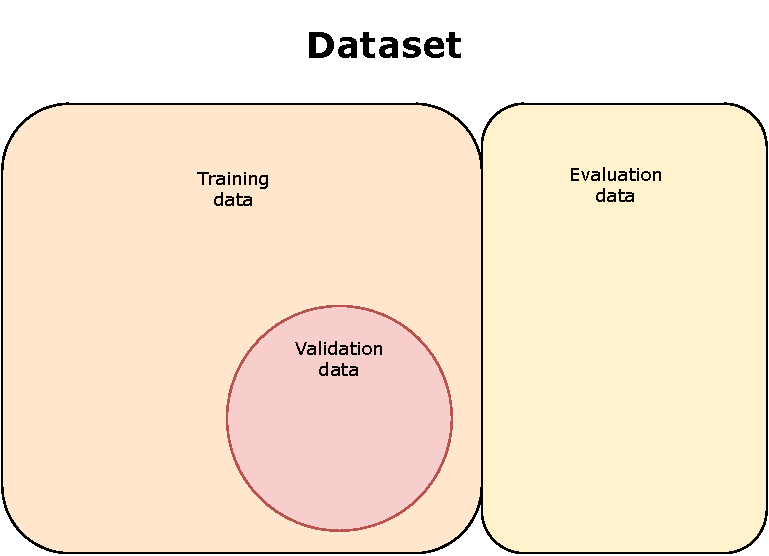
\includegraphics{img/train_test_data.pdf}
  \caption{Visualization of a dataset evaluation split. Training and evaluation data are subsets of the dataset, and the validation data is a subset of the training data.}
  \label{figure:dataset_train_test}
\end{figure}

It is common to split the inputs and output data into multiple parts, where some of the data is used to test the model. Testing of the model can happen at different times: after training sessions (evaluation) and in between epochs (validation). 

Before starting a model training session, we split the dataset into training and evaluation data, where the first part is what the model is trained to fit, and evaluation data is kept aside until the training is complete. Then we use it to check the performance of the trained model. Metrics used here is the value of the loss function (for example mean squared error) for value prediction, or classification metrics described above.

Validation data and is useful to include when we are developing the model, as we regularly see how the model is performing after each epoch. The metric used is usually the value of the loss function or the accuracy score, depending on the objective of the model. When the model is good enough for the desired task, we do not need validation data. We pass the validation split into the function that starts the model's training as either the validation\_split or the validation\_data parameter. If the validation\_split parameter is used (a number between 0 and 1), the validation data is calculated automatically before training starts. If, however, we want to use specific samples as validation data, we use the validation\_data parameter instead.

The function \textit{train\_test\_split} from the \textit{sklearn} package is useful to split up the dataset into training and evaluation data. We input dataset (X, y), plus how large we want the training and test sets to be (number between 0 and 1, which determines the size of the test partition). The function also randomizes the data, preventing model to accidentally learn something correct for segments in a row that also are chronologically in order. After calling the function, you end up with two arrays for input data (\textit{X\_train, X\_test}), and two arrays for output data (\textit{y\_train, y\_test}). In this case the \textit{test\_size} is set to $0.4$, meaning that the test set contains $40\%$ of the total dataset and the remaining $60\%$ are in the training set.

\begin{figure}[h]
\begin{code}
    \begin{minted}[linenos]{python}
from sklearn.model_selection import train_test_split

X_train, X_test, y_train, y_test = train_test_split(X, y, 
                                                    test_size=0.4)
    \end{minted}
    \caption{Sklearn train and test split. After calling this function we end up with training and testing sets for both inputs and outputs.}
    \label{code:sklearn_train_test_split}
\end{code}
\end{figure}

\begin{figure}[h]
  \begin{code}    
      \begin{minted}[linenos]{python}
      from sklearn.model_selection import StratifiedKFold
  
      X, y = load_data(...)
  
      skf = StratifiedKFold(n_splits=3, shuffle=True)
  
      for train_index, test_index in skf.split(X, y):
          X_train, X_test = X[train_index], X[test_index]
          y_train, y_test = y[train_index], y[test_index]
  
          model = create_model(...)
          model.fit(X_train, y_train, ...)
          results = model.evaluate(X_test, y_test)
  
          # do something with results...
  
      \end{minted}
      \caption{StratifiedKFold from sklearn. The dataset is split in 3 parts (n\_splits on line 5), then training and evaluation happens for each of the parts.}
      \label{code:sklearn_k_fold}
  \end{code}
\end{figure}
  

\subsubsection{Cross-validation}
Another popular choice is to use something called \textit{K-fold cross-validation}. It works by splitting the dataset into $K$ train and test sets, and for each of them, train the model on the training set and validate on the test set. Cross-validation is a good way of checking if your model's performance truly is independent on which data samples it trained on. The higher number of splits ($K$) means fewer data samples to test on, so you need to keep that in mind (the same for \textit{train\_test\_split} if you set the \textit{test\_size} too low). Sklearn has an implementation of \textit{K-fold}, called \textit{StratifiedKFold}. An example of how it can be used is shown in code \ref{code:sklearn_k_fold}, where we perform a 3-fold cross-validation ($K = 3$). 

Performance testing of a model sometimes happens with both train/test-split and cross-validation. We set aside a small part of the dataset for evaluation and generating folds for the rest, then within each fold, we train and validate the model, and evaluate it against the part of the dataset that we set aside at the beginning. We note loss/accuracy scores for each fold and calculate the mean value which is the overall performance result.

Another way of using cross-validation to test the performance of a model is by leaving N participants out of the dataset. We do this by generating training data for the rest of the participants and evaluation data for the N participants left out. We log the performance scores for each fold, and then we find the overall average. 

In this thesis, we will use all described methods of splitting training and testing data. Simple train/test splitting is what we begin with during the development of the models. Then we perform cross-validation to verify that the models are consistent, and finally, we leave participants out one by one. The latter is essentially the same as 55-fold cross-validation, and it is a way of comparing our work to the work of Garcia-Ceja, E. et al., where they also evaluated their models by leaving participants out one by one \cite{GarciaCeja2018_classification_bipolar}. 

\begin{figure}
\begin{center}
  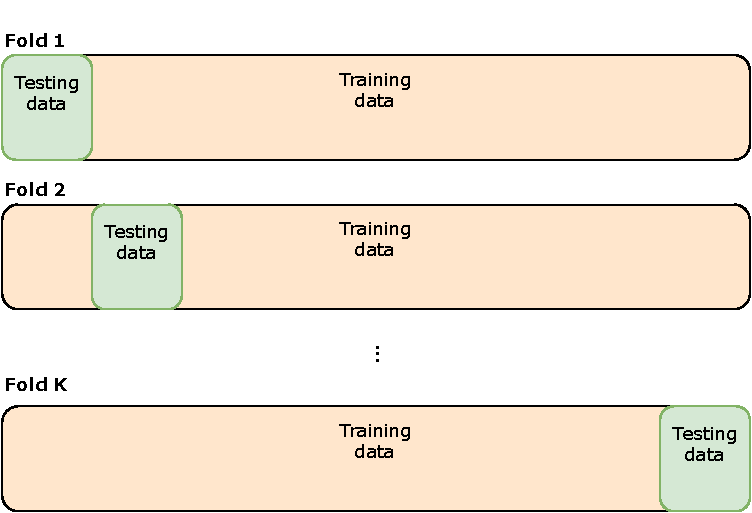
\includegraphics{img/Cross-validation.pdf}
  \caption{K-fold cross-validation visualized. For each fold, a testing set is defined, and the rest of the data is a training set.}
  \label{figure:dataset_cross_val}
\end{center}  
\end{figure}